% !TEX root =  ../master.tex
\chapter{Anforderungsanalyse} % TODO: Das hier ist noch etwas durcheinander
\section{Abgrenzung}
\subsection{Abgrenzung des Funktionsumfangs}
Im bereich Bildung gibt es viele Möglichkeiten, wie Hochschulen und Studenten unterstützt werdem können.
Primär gibt es hierbei 4 Ebenen, auf der Aktionen stattfinden können:
\begin{itemize}
    \item Politische Ebene\\
        Landesweite Veränderungen, die das gesamte Bildungssystem betreffen 
    \item Institutionsebene\\
        Veränderungen an der gesamten Bildungseinrichtung.
    \item Kursebene\\
        Aktionen innerhalb eines Kurses bzw. Vorlesung
    \item Individualebene\\
        Persönliche Veränderungen
\end{itemize}
Man kann ableiten, dass sich nicht alle Ebenen gleich für die zu entwickelnde Anwendung anbieten.
Auf politischer Ebene veränderungen durchzusetzen benötigen in der Regel ein aufwändiges Genehmigungsverwähren, welches wertvolle Zeit in Anspruch nehmen.
Da die Anwendung aber möglichst schnell Krisenbeeinträchtigte Studenten unterstützt werden sollen, muss diese Ebene bei der Entwicklung zunächst vernachlässigt werden.

Die Institutionsebene beschreibt das Management von Ressourcen innerhalb der Hochschule.
Besonders der Austauch und Weiterbildung zwischen Dozenten ist hierbei ein wichtiger Aspekt.
Problematisch ist aber die Identifizierung von Anforderungen aller Studienrichtungen.
So besitzen technische Studiengänge andere Bedürfnisse als wirtschaftlich orientierte Studiengänge.
Aus diesem Grund kann auch diese Ebene nicht genauer beachtet werden.

Stattdessen wird sich in dieser Arbeit auf die Entwicklung einer Anwendung mit dem Schwerpunkt auf der Kurs- und der Individualebene fokussiert.
Die Kursebene dient zur Weitergabe Lernmaterialien, die eine Vorlesung ergänzen.
Dies soll einen direkten Einfluss auf die Individualebene haben und den individuellen Studenten fördern.
Ziel ist es den Studenten beim Lernen zur unterstützen und das Verständnis der in der Vorlesung vermittelten Informationen zu fördern.  

\begin{figure}[]%FIXME:
    \begin{center}
        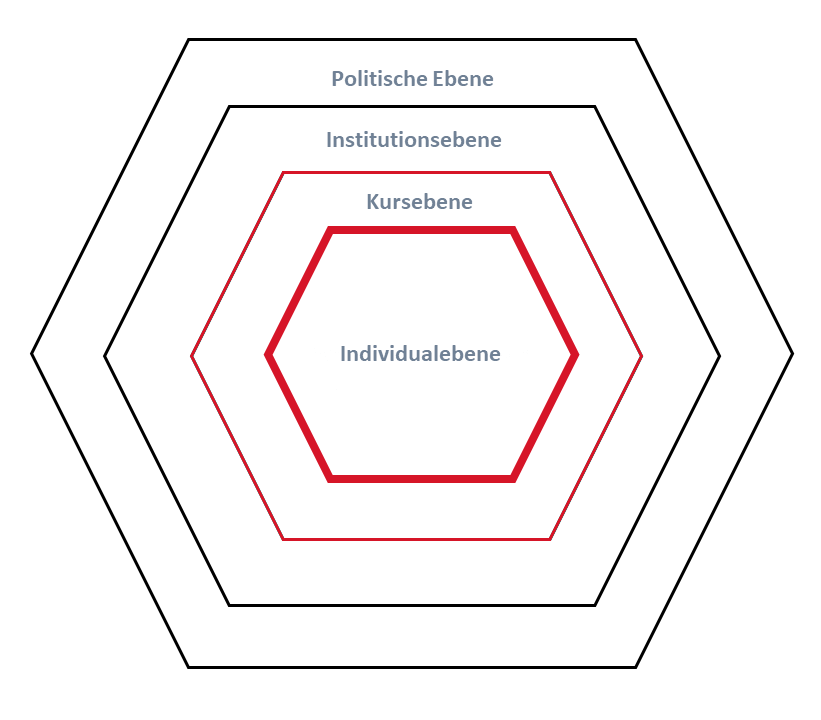
\includegraphics[width=.7\textwidth]{img/Ebenen.png}
        \caption{Aktionsebenen}
        \label{fig:ebenen}
    \end{center}
\end{figure}
%TODO: Verweis auf pptx Fr. Honal % TODO: Gibt es hier noch Quellen?

Durch diesen Fokus entfallen allerdings Vorteile, die sich durch eine größere Nutzer- und damit Datenbasis ergeben.
Besonders die Möglichkeit für Datenanalysen als Teil des Data Minings ist aufgrund des geringen Datenumfangs nicht möglich.
Gleichzeitig sind wir der Überzeugung, dass eine Auswertung des Lernfortschrittes nicht der primäre Grund für die Entwicklung einer Anwendung sein sollte, sondern der Mehrgewinn für Studenten.
Sollte sich die Anwendung für Nutzer als Vorteilhaft erweisen, kann die Anwendung ohne Probleme um Funktionalitäten aus anderen Ebenen erweitert werden.



% TODO: Können Wir vielleicht noch einen User Acceptance Test machen?

% Um eine Fortführung und Integration der anderen Ebenen in Zukunft zu ermöglichen, soll die Datenhaltung und Architektur der Anwendung so konzipiert werden, dass eine Erweiterung leicht möglich ist.

% TODO: Also bauen wir einen Export? Das wäre gut, dann können wir das schreiben. Aber da müssen wir mal schauen. Vordefinierte Auswertungen, Berechnungen wird es allerdings aufgrund der gewählten Abgrenzungen erst einmal nicht geben.
% Die vorhandenen Daten sollen im Ersten Schritt in einem auswertungstauglichen Format zur Verfügung gestellt werden.
% Die Auswertung selbst muss durch den Dozenten selbst erfolgen.

% TODO: Abgrenzung zu anderen Werkzeugen
\subsection{Abgrenzung zu anderen Anwendungen}
Im Hochschulkontext kommen bereits mehrere Systeme zum Einsatz.
Die primäre Plattform bildet \enquote{Moodle}.
% TODO: Moodle

Eine weitere Plattform, die verwendet wird ist Dualis
% TODO: Dualis

% TODO: MyLA


\section{Ist-Analyse}
Grundlage dieser Arbeit ist die Vision der DHBW, Learning Analitics weiter voranzutreiben.
Aus Datenschutzrechtlichen Gründen, wird aktuell die Learning Analytics Erweiterungen und Möglichkeiten der Kursmanagement und Lernplattform Moodle nicht genutzt.
Aus einem bereits umgesetzten Projekt ist ein Prototyp entstanden, der es ermöglichen soll Daten im Verlauf der Vorlesungen mit der Hilfe von Umfragen zu generieren.
Weitere Infos über das Projekt und deren Ergebnisse können hier (https://github.com/dhbw-myla/myla) nachgelesen werden. 
Die dabei entsandene Webanwendung ermöglicht es Umfragen zu erstellen, zu verwalten und auszuwerten.
Für Dozenten gibt es die Möglichkeit, Umfragen zu erstellen und mit ihren Studierenden zu teilen.
Diese haben dadurch die Chance, ihre Meinung zur Vorlesung mitzuteilen, Gelerntes zu verinnerlichen oder auch um Anmerkungen zu gestellten Fragen zu geben.
Die Plattform ermöglicht es dabei, Umfragen als Vorlage zu speichern, sodass diese in unterschiedlichen Kursen verwendet werden können und zeigt die Ergebnisse der Umfragen graphisch an.
Allerdings ist anzumerken, dass wir in unserem Studium neben der Vorstellung der Anwendung für unser Projekt nie mit der Anwendung gearbeitet hatten und diese nach aktuellem Wissensstand auch nicht von der DHBW gehostet wird, was eine breite Nutzung eher unwahrscheinlich macht. 



\section{Funktionale Anforderungen} % TODO: Vielleicht stichpunkte? Ich fands etwas schwer zu lesen
Problematisch bei der Meinungserhebung mittels Umfragen ist häufig die Art und Formulierung der Fragestellung, das Nichtbeantwortungsproblem und ggf. mangelnde Repräsentativität.
Mehr Hintergründe und Lösungsansätze zu diesen und weiteren Problemen lassen sich in der Einschlägigen Fachliteratur nachlesen.
Ziel dieser Arbeit ist es diesen Probleme entgegen zu Wirken, in dem wir eine Anwendung entwickeln, die auch einen direkten Mehrwert für die Studenten hat.
Zwar erbringt die Datenerhebung und Auswertung mittels Umfragen langfristige Mehrwerte, bei der Teilnahme an der Umfrage entsteht jedoch erst einmal ein Aufwand, dessen Nutze ungewiss ist.
Aus diesem Grund ist das Motto "Von Studenten für Studenten" entstanden.
Wir als Studenten der DHBW können sehr gut einschätzen was uns das Studium erleichtern würde und wie wir uns in Bezug auf Klausuren und Prüfungen organisieren.
Mit einer Prozessierung und Automatisierung können Synergien genutzt werden und auch andere Kommilitonen von den für diese Veranstaltungen eingebrachten Aufwänden profitieren. 

Ziel dieser Arbeit ist es eine App zu entwickeln, die Plattform unabhängig als Web-Applikation oder im Browser genutzt werden kann.
Dabei sollen sowohl Studenten als auch Dozenten einen Zugang bekommen.
Um eine möglichst hohe Nutzerzahl erreichen zu können, setzen wir auf eine freiwillige Teilnahme.
Die Anwendungen soll durch ihre Funktionen und die intuitive Bedienbarkeit überzeugen und nicht durch einen Nutzungszwang.
Zweiteres würde unserer Einschätzung nach nur zu einer halbherzigen Nutzung führen, was in einer schlechteren Datenqualität enden würde und damit Auswertungen und deren Interpretation erschweren würde. 

Bei der Erstanmeldung sollen bereits erste Daten über den Lerntyp der Studenten gestellt und gespeichert werden.
Besitzt ein Nutzer einen Account, soll er Kurse anlegen können, zu denen er Informationen wie Datum von Prüfungen erfassen kann.
Für jeden Kurs besteht die TODOs mit Zeildatum zur Strukturierung der eigenen Arbeit anzulegen.
Außerdem können für eine bessere Prüfungsvorbereitungen Karteikarten angelegt werden.
Die Karteikarten können auch in der App gelernt werden.
Dabei soll auf wissenschaftlich fundierte Algorithmen zurückgegriffen werden, die das Lernen erleichtern sollen und dafür sorgen, dass sich das gelernte auch im Langzeitgedächtnis festigt.
Dies ist aus eigenen Erfahrungen in den meist Stressigen Klausurenphasen leider nicht der Fall.
Außerdem sollen die eingetragenen TODOs graphisch angezeigt werden, sodass eine Art Kalender entsteht und Kapazitätsengpässe rechtzeitig erkannt und durch Umplanen verhindert werden können.
Um zu verhindern, dass diese organisatorische Aufwand von jedem Studenten einzeln durchgeführt werden müssen soll es zusätzlich die Funktion geben, dass Dozenten einen Kurs anlegen können.
Diesen können Sie dann mit der Hilfe eines Einschreibeschlüssels unter ihren Studierenden teilen.
Den Kursen können initial bereits Prüfungstermine, TODOs und Karteikarten mitgegeben werden.
Somit entfällt die initiale Erstellung.
Die zu einem Kurs gehörenden Informationen können von den Studierenden weiterhin nach belieben angepasst und ergänzt werden ohne dabei für die anderen eingeschriebenen Kursteilnehmer Daten zu verändern.
Das Erstellen eines Kurses hat für den Dozenten den Vorteil, dass für diesen Kurs Daten zur Verfügung gestellt bekommt, die er zur Anpassung oder Evaluation seiner Vorlesung nutzen kann.
Beispiele hierfür können sein Lerntypen der Studenten, Fortschritt beim Lernen der Karteikarten, etc.
Wichtig ist dabei anzumerken, dass diese Daten vollständig anonym ohne Verweise auf Personen oder andere Identifikationsmerkmale zur Verfügung gestellt werden, sodass auch keine Probleme mit dem Datenschutz vorliegen. 



\section{Nicht-Funktionale Anforderungen}




% TODO: Und dann am schluss noch eine Zusammenfassungstabelle



% TODO: Irgendwo auch ncohaml sagen, dass man erst einen nutzer nutzen haben buss, bevor man daten minen kann. Ohne nutzer /funktionen macht es gar keinen sinn